\section{Model Selection \& Final Pipeline}

After the feature set settled down, the model story became much cleaner. Single models were good enough to guide the search, but the best public path came from letting several branch families vote in different ways:
\begin{enumerate}
    \item XGBoost on the engineered numeric matrix.
    \item LightGBM on the same processed frame.
    \item CatBoost on the mixed feature table with categorical columns preserved.
    \item ExtraTrees as a strong but simpler diversity branch.
    \item An MPS neural branch to add a different error profile.
\end{enumerate}

Instead of freezing mysterious blend weights inside the report code, the public repo now reads the original tuned branch configurations from saved overnight artifacts and fits the blend/meta combiner openly in code. That is closer to how the actual project worked and much easier to explain.

\begin{table}[H]
    \centering
    \small
    \begin{tabular}{@{} l c c c @{}}
        \toprule
        Model & Accuracy & \(R^2\) & Combined \\
        \midrule
        \texttt{meta\_overnight} & 0.8477 & 0.8513 & \textbf{0.8495} \\
        \texttt{blend\_overnight} & 0.8424 & 0.8485 & 0.8455 \\
        \texttt{target\_stats\_blend} & 0.8563 & 0.8552 & 0.8557 \\
        \texttt{mlp\_meta\_stack\_v1} & 0.8587 & 0.8556 & 0.8572 \\
        \texttt{mlp\_weighted\_blend\_v1} & 0.8600 & 0.8553 & \textbf{0.8576} \\
        \bottomrule
    \end{tabular}
    \caption{Representative validation checkpoints from the project.}
    \label{tab:model-table}
\end{table}

\begin{figure}[H]
    \centering
    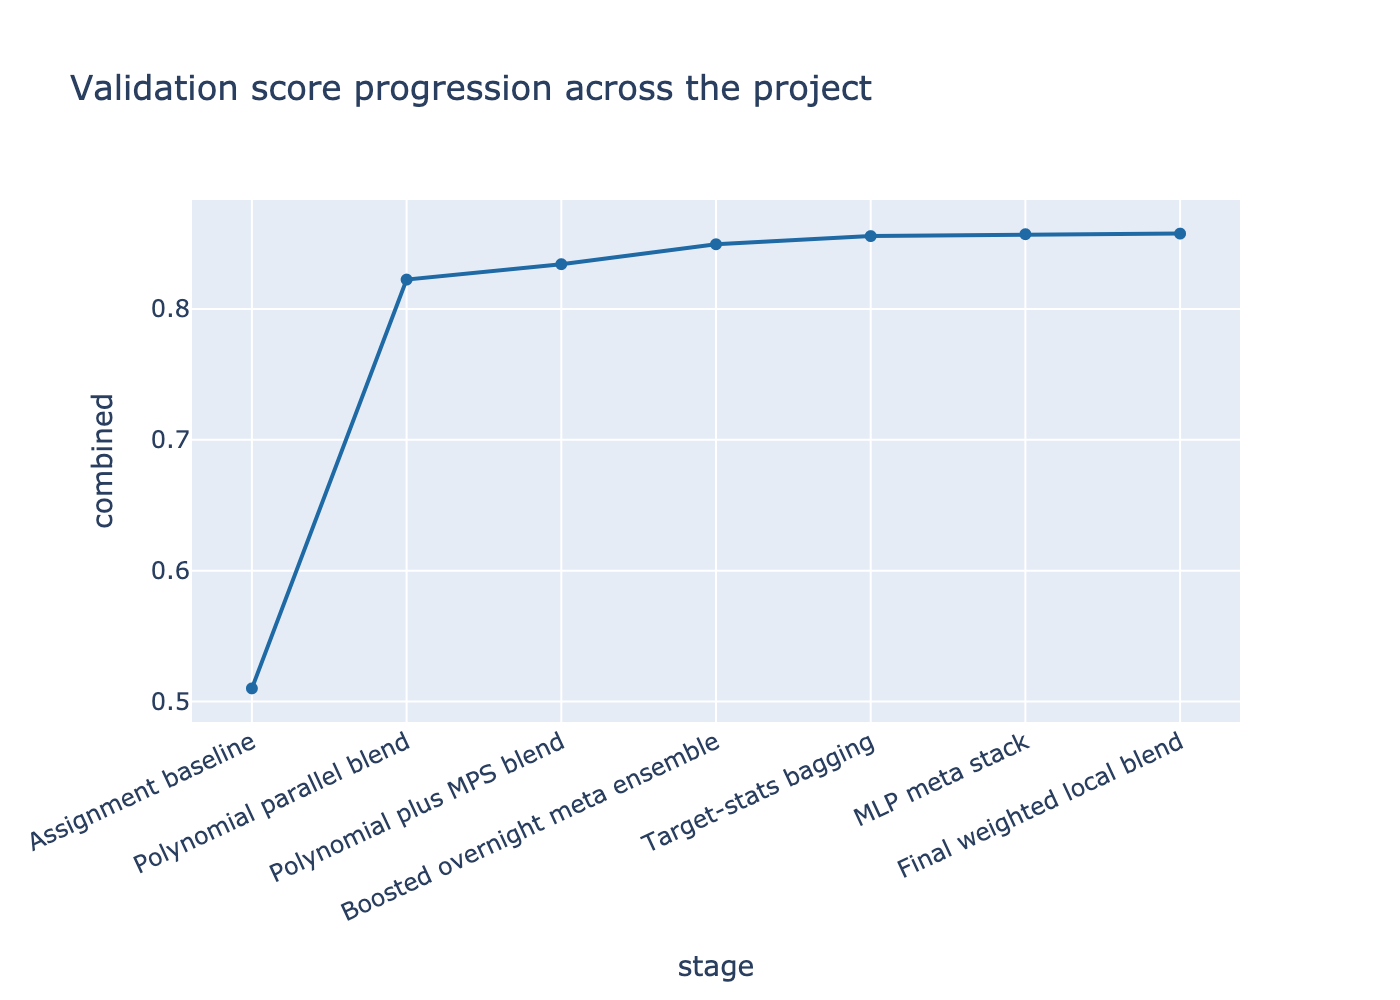
\includegraphics[width=0.86\linewidth]{figures/stage_progress.png}
    \caption{The project kept improving after the public-best lane, but those later gains came from heavier local-only combinations rather than a cleaner public submission path.}
    \label{fig:stage-progress}
\end{figure}

The final choice was mostly a trade-off between clarity and squeezing out the last few thousandths. We did reach a stronger local score later, but that route was harder to present cleanly and harder to justify as the main public notebook. For the repo and the report, \texttt{meta\_overnight} is the right landing point: strong score, readable branch structure, and a direct path from raw CSVs to a final submission file.
